%-------------------------------------------------------
\section{Ecossistema Docker}
%-------------------------------------------------------

\subsection{Docker Hub/Store}
\begin{frame}[fragile]{Ecossistema}{Docker Hub/Store}
  \begin{figure}[ht!]
    \centering
    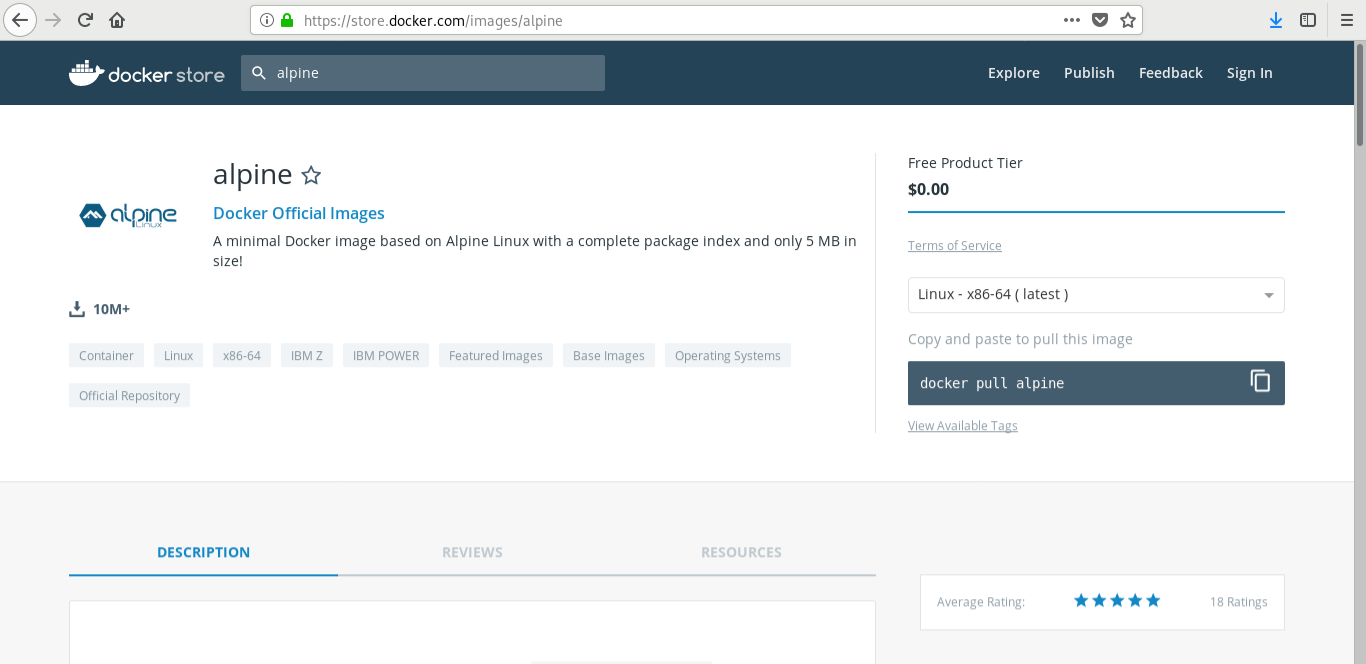
\includegraphics[width=110mm]{images/hub_store.png}
  \end{figure}
  \begin{lstlisting}[language=bash]
  # bash console
  docker push $DOCKER_ID_USER/minha_primeira_imagem:share
  \end{lstlisting}
\end{frame}

\subsection{Docker Registry}
\begin{frame}[fragile]{Ecossistema}{Docker Registry}
  Registro (registry) é um repositório para armazenamento e distribuição de imagens.
  \begin{figure}[ht!]
    \centering
    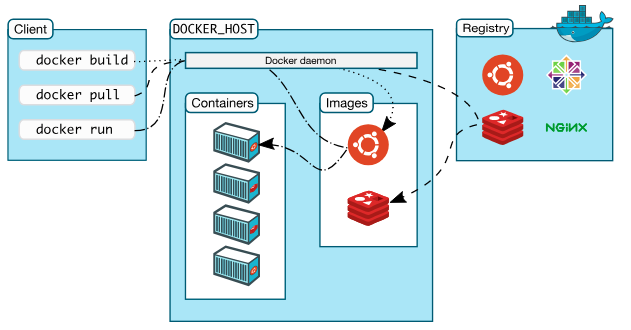
\includegraphics[width=90mm]{images/architecture.png}
  \end{figure}
  \begin{lstlisting}[language=bash]
  # bash console
  docker build -t ubuntu:share .
  docker pull redis
  docker run --name ubuntu_share ubuntu:share
  \end{lstlisting}
\end{frame}

\subsection{Docker Machine}
\begin{frame}{Ecossistema}{Docker Machine}
  \begin{figure}[ht!]
    \centering
    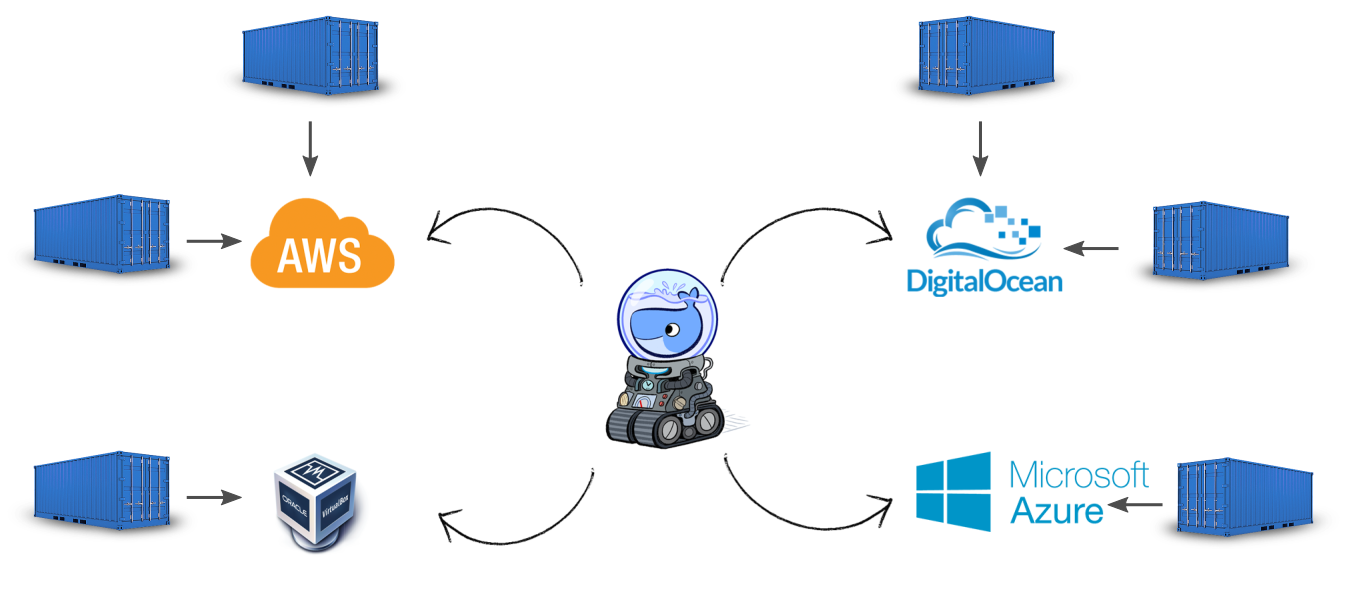
\includegraphics[width=100mm]{images/docker_machine}
  \end{figure}
  Docker machine é a ferramenta usada para gerência distribuída, permite a instalação e gerência de docker hosts de forma fácil e direta.
\end{frame}

\subsection{Docker Swarm}
\begin{frame}{Ecossistema}{Docker Swarm}
  \begin{figure}[ht!]
    \centering
    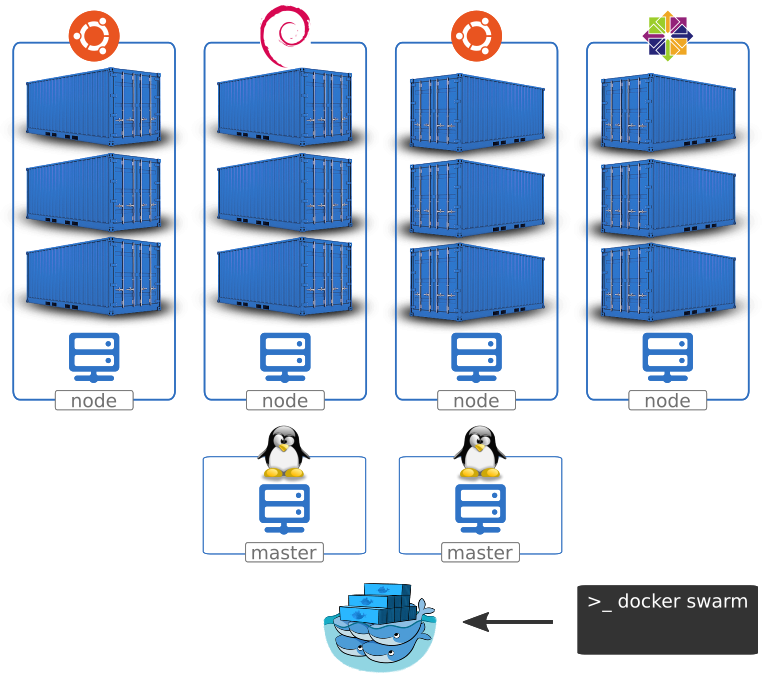
\includegraphics[width=60mm]{images/docker_swarm}
  \end{figure}
  O Docker Swarm permite que containers executem distribuídos em um cluster, controlando a quantidade de containers, balanceamento de carga, registro, deploy, replicas e update de serviços.
\end{frame}

\subsection{Docker Compose}
\begin{frame}{Ecossistema}{Docker Compose}
  \begin{figure}[ht!]
    \centering
    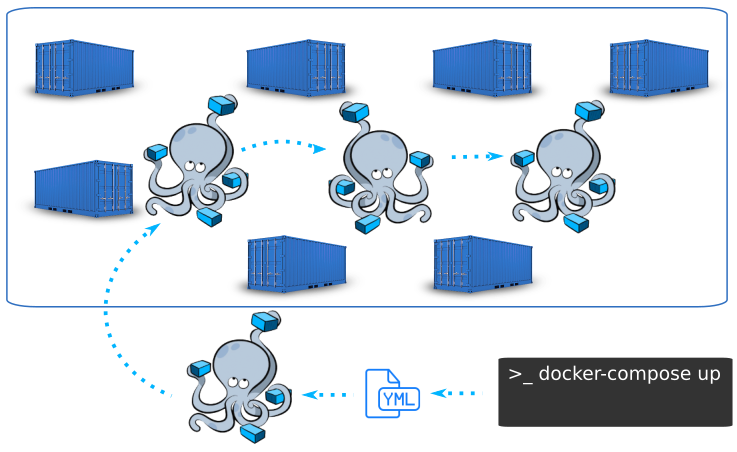
\includegraphics[width=80mm]{images/docker_compose}
  \end{figure}
  Docker Compose é um orquestrador de containers da Docker, facilita a criação e administração de um conjunto de containers a partir do uso de um simples arquivo de configuração em formato YAML.
\end{frame}

\begin{frame}[fragile]{Ecossistema}{Docker Compose}
  \begin{itemize}
    \item<1-> Docker-compose
  \end{itemize}
  \begin{lstlisting}[language=docker]
  version: '3'

  services:
    web:
      build: .
      ports:
       - "9090:5000"
      volumes:
       - .:/code
    redis:
      image: "redis:alpine"
  \end{lstlisting}
  \begin{lstlisting}[language=bash]
  # bash console
  docker-compose up
  \end{lstlisting}
\end{frame}

\begin{frame}[fragile]{Exemplo}{Docker Compose}
  \begin{figure}[ht!]
    \centering
    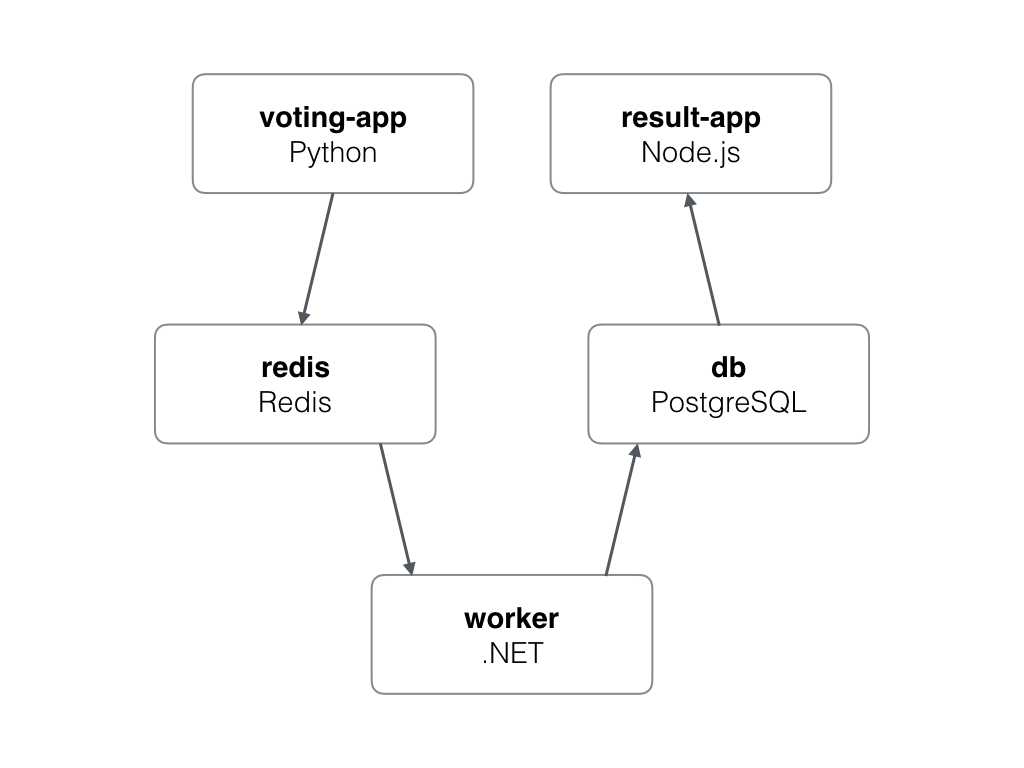
\includegraphics[width=80mm]{images/vote_app.png}
  \end{figure}
  \begin{lstlisting}[language=bash]
  # bash console
  docker-compose up -d
  \end{lstlisting}
\end{frame}